%!TEX root = ../report.tex
\documentclass[../report.tex]{subfiles}

\begin{document}
\section{Methodology}
\label{sec:methodology}

\subsection{LLM Cognition}
[TODO]

\subsection{Simulation}
The agent and its environment were simulated using the PyBullet physics engine. As PyBullet is a Python module, it's functionality can be directly integrated in any python script. This allows precise control over the simulation and its interaction with external tool calls. PyBullet also comes with methods to create custom objects as well as a fully implemented robotic arm, the KUKA iiwa model. These methods and the KUKA iiwa robotic arm where used to create the agents embodiment and the environment it can act in. \\
The agent's body is modeled as a mobile manipulator, consisting of a square omnidirectional base and a 7-DoF robotic arm derived from the KUKA iiwa model.
To increase maneuverability, the rotational joint limits of the arms joint connecting the base to the arm were disabled, enabling full 360° reach around the base. A fully articulated gripper was not implemented. Instead, grasping and placing were simplified by attaching objects directly to the end-effector when within a predefined proximity threshold, and detaching them at the desired placement location. Figure \ref{fig:agent} depicts the agent.

\begin{figure}[h!]
	\centering
	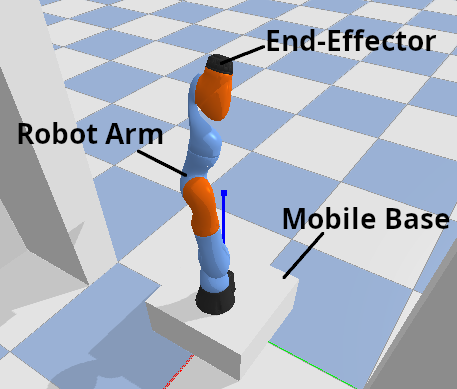
\includegraphics[width=0.45\textwidth]{figures/agent.png}
	\caption{The simulated mobile manipulator consisting of a square omnidirectional base and a 7-DoF arm.}
	\label{fig:agent}
\end{figure}

The environment was designed as a simplified two-room household, comprising a kitchen and a living room. The kitchen contains a three-layer shelf and a table, both capable of supporting objects. The living room contains a television placed on a table. The two rooms are connected by a hallway. Figure \ref{fig:environment} shows the environment and the semantic map used for navigation. The green dots are locations the agent can navigate to via the connected lines.

\begin{figure}[h!]
	\centering
	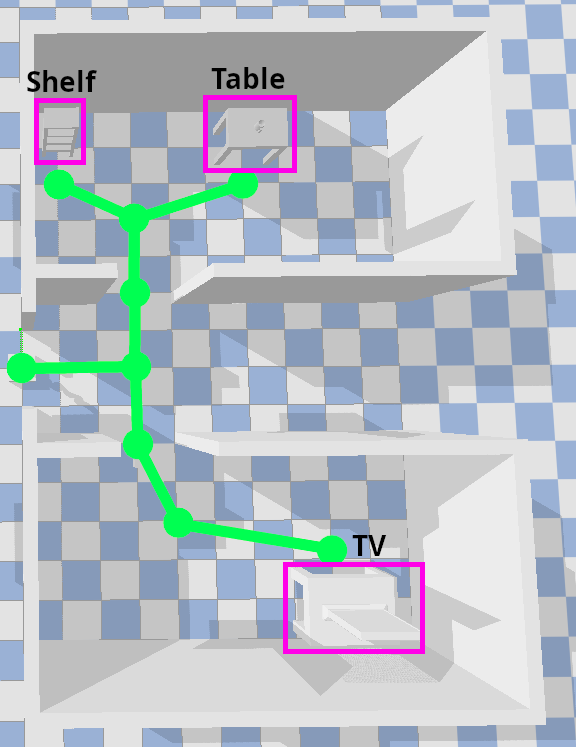
\includegraphics[width=0.45\textwidth]{figures/environment.png}
	\caption{The simulated household environment and its semantic map representation consisting of a kitchen, a living room, and a connecting hallway.}
	\label{fig:environment}
\end{figure}

To interact with the environment and its objects, the agent was equipped with several tool functions, each exposed through a tool-calling interface with text-based status responses. The implemented tools are summarized below:
\begin{itemize}
	\item \textbf{Look around:} Returns the agent's location on a semantic map of the environment, as well as a list of objects detected in proximity of the agent and where these objects are placed.
	\item \textbf{Query Memory:} The agent queries its episodic memory to gain information from prior executions of the task.
	\item \textbf{Move To:} Executes navigation to a goal location on the semantic map. Path planning is performed using the A* algorithm; if a valid path is found, the agent follows it until the goal is reached. If no path is available, the tool reports failure.
	\item \textbf{Grab:} Moves the robot arm toward a specified target object. If the end-effector reaches within a proximity threshold, the object is attached to the arm, and the tool reports success. Failure is reported if the target object does not exist, is out of reach, or if the agent is already holding an object.
	\item \textbf{Place:} Allows the agent to release the currently held object at a specified location. Placement succeeds if the end-effector reaches the designated location, the location is unoccupied, and the agent is holding an object. Otherwise, the tool reports failure, specifying the violated condition.
	\item \textbf{Scratch Pad:} The agent can write in lenght about anything it wants to reason about. This allows the agent to plan its actions beforehand.
	\item \textbf{Summarize Task:} The agent provides a summary of an atempted task, including if it succeded or failed and what actions it did or attempt to complete the task.
\end{itemize}

\end{document}
